\documentclass{article}
\usepackage{fancyhdr}
\usepackage{extramarks}
\usepackage{amsmath}
\usepackage{amsthm}
\usepackage{amsfonts}
\usepackage{tikz}
\usepackage[plain]{algorithm}
\usepackage{algpseudocode}
\usepackage{listings} 
\usepackage{neuralnetwork}
\usepackage{subfigure}
\usepackage{xltxtra,fontspec,xunicode}
\usepackage[slantfont,boldfont]{xeCJK} % 允许斜体和粗体
\usepackage{xeCJK}
\setCJKmainfont{PingFangSC-Regular}   % 设置缺省中文字体
\setCJKmonofont{Hei}   % 设置等宽字体
% \setmainfont{Optima}   % 英文衬线字体
\setmonofont{FiraCode-Regular}   % 英文等宽字体
% \setsansfont{Trebuchet MS} % 英文无衬线字体
\usetikzlibrary{automata,positioning}

\usepackage{color}
\definecolor{dkgreen}{rgb}{0,0.6,0}
\definecolor{gray}{rgb}{0.5,0.5,0.5}
\definecolor{mauve}{rgb}{0.58,0,0.82}

\lstset{frame=tb,
  language=Python,
  aboveskip=3mm,
  belowskip=3mm,
  showstringspaces=false,
  columns=flexible,
  basicstyle={\small\ttfamily},
  numbers=none,
  numberstyle=\tiny\color{gray},
  keywordstyle=\color{blue},
  commentstyle=\color{dkgreen},
  stringstyle=\color{mauve},
  breaklines=true,
  breakatwhitespace=true,
  tabsize=3
}
%
% Basic Document Settings
%

\topmargin=-0.45in
\evensidemargin=0in
\oddsidemargin=0in
\textwidth=6.5in
\textheight=9.0in
\headsep=0.25in

\linespread{1.1}

\pagestyle{fancy}
\lhead{\hmwkAuthorName}
\chead{\hmwkClass\: \hmwkTitle}
\rhead{\firstxmark}
\lfoot{\lastxmark}
\cfoot{\thepage}

\renewcommand\headrulewidth{0.4pt}
\renewcommand\footrulewidth{0.4pt}

\setlength\parindent{0pt}

%
% Create Problem Sections
%

\newcommand{\enterProblemHeader}[1]{
    \nobreak\extramarks{}{Task \arabic{#1} continued on next page\ldots}\nobreak{}
    \nobreak\extramarks{Task \arabic{#1} (continued)}{Problem \arabic{#1} continued on next page\ldots}\nobreak{}
}

\newcommand{\exitProblemHeader}[1]{
    \nobreak\extramarks{Task \arabic{#1} (continued)}{Problem \arabic{#1} continued on next page\ldots}\nobreak{}
    \stepcounter{#1}
    \nobreak\extramarks{Task \arabic{#1}}{}\nobreak{}
}

\setcounter{secnumdepth}{0}
\newcounter{partCounter}
\newcounter{homeworkProblemCounter}
\setcounter{homeworkProblemCounter}{1}
\nobreak\extramarks{Task \arabic{homeworkProblemCounter}}{}\nobreak{}

%
% Homework Problem Environment
%
% This environment takes an optional argument. When given, it will adjust the
% problem counter. This is useful for when the problems given for your
% assignment aren't sequential. See the last 3 problems of this template for an
% example.
%
\newenvironment{homeworkProblem}[1][-1]{
    \ifnum#1>0
        \setcounter{homeworkProblemCounter}{#1}
    \fi
    \section{Task \arabic{homeworkProblemCounter}}
    \setcounter{partCounter}{1}
    \enterProblemHeader{homeworkProblemCounter}
}{
    \exitProblemHeader{homeworkProblemCounter}
}

%
% Homework Details
%   - Title
%   - Due date
%   - Class
%   - Section/Time
%   - Instructor
%   - Author
%

\newcommand{\hmwkTitle}{Lab\ \#5}
\newcommand{\hmwkDueDate}{September 25, 2019}
\newcommand{\hmwkClass}{CSCI964 Computational Intelligence}
\newcommand{\hmwkClassTime}{3.5}
\newcommand{\hmwkClassInstructor}{Zhifeng Wang}
\newcommand{\hmwkAuthorName}{\textbf{Mei Wangzhihui}}
\newcommand{\hmwkAuthorNum}{\textbf{2019124044}}
%
% Title Page
%

\title{
    \vspace{2in}
    \textmd{\textbf{\hmwkClass:\ \hmwkTitle}}\\
    % \normalsize\vspace{0.1in}\small{Due\ on\ \hmwkDueDate\ at 3:10pm}\\
    % \vspace{0.1in}\large{\textit{\hmwkClassInstructor\ \hmwkClassTime}}
    \vspace{3in}
}

\author{\hmwkAuthorName\ \hmwkAuthorNum}
\date{}

\renewcommand{\part}[1]{\textbf{\large Part \Alph{partCounter}}\stepcounter{partCounter}\\}

%
% Various Helper Commands
%

% Useful for algorithms
\newcommand{\alg}[1]{\textsc{\bfseries \footnotesize #1}}

% For derivatives
\newcommand{\deriv}[1]{\frac{\mathrm{d}}{\mathrm{d}x} (#1)}

% For partial derivatives
\newcommand{\pderiv}[2]{\frac{\partial}{\partial #1} (#2)}

% Integral dx
\newcommand{\dx}{\mathrm{d}x}

% Alias for the Solution section header
\newcommand{\solution}{\textbf{\large Solution}}

% Probability commands: Expectation, Variance, Covariance, Bias
\newcommand{\E}{\mathrm{E}}
\newcommand{\Var}{\mathrm{Var}}
\newcommand{\Cov}{\mathrm{Cov}}
\newcommand{\Bias}{\mathrm{Bias}}

\begin{document}

\maketitle

\pagebreak

\begin{homeworkProblem}
\begin{lstlisting}
    '''
@Author: maywzh
@Date: 2020-03-21 14:14:43
@FilePath: /ji_coursenotes/2020spring/CSCI964/lab5-0323/src/kmeans.py
'''
import numpy as np
import random
import re
import matplotlib.pyplot as plt


def loadDataSet(filename):
    """数据读取."""
    dataSet = np.loadtxt(filename, delimiter=',', usecols=(0, 1, 2, 3))
    return dataSet


def initCentroids(dataSet, k):
    """初始化k个簇心"""
    dataSet = list(dataSet)
    return random.sample(dataSet, k)


def getCentroids(clusterDict):
    """重新计算k个簇心"""
    centroidList = []
    for key in clusterDict.keys():
        centroid = np.mean(clusterDict[key], axis=0)
        centroidList.append(centroid)
    return centroidList


def calcuDistance(vec1, vec2):
    """计算两点间的欧式距离"""
    return np.sqrt(np.sum(np.square(vec1 - vec2)))


def getMSE(centroidList, clusterDict):
    """计算各簇集合间的均方误差 将簇类中各个点与簇心的距离累加求和"""
    sum = 0.0
    for key in clusterDict.keys():
        vec1 = centroidList[key]
        distance = 0.0
        for item in clusterDict[key]:
            vec2 = item
            distance += calcuDistance(vec1, vec2)
        sum += distance
    return sum


def minifyDistance(dataSet, centroidList):
    """
    基于选定k个簇心,重新聚簇
    """
    clusterDict = dict()
    k = len(centroidList)
    for item in dataSet:
        vec1 = item
        flag = -1
        minDis = float("inf")
        for i in range(k):
            vec2 = centroidList[i]
            distance = calcuDistance(vec1, vec2)
            if distance < minDis:
                minDis = distance
                flag = i  # 循环结束时, flag保存与当前item最近的蔟标记
        if flag not in clusterDict.keys():
            clusterDict.setdefault(flag, [])
        clusterDict[flag].append(item)  # 加入相应的类别中
    return clusterDict  # 不同的类别


def showCluster(centroidList, clusterDict):
    """可视化聚类结果
    """
    colorMark = ['or', 'ob', 'og', 'ok', 'oy', 'ow']  # 不同簇类标记,o表示圆形,另一个表示颜色
    centroidMark = ['dr', 'db', 'dg', 'dk', 'dy', 'dw']

    for key in clusterDict.keys():
        plt.plot(centroidList[key][0], centroidList[key]
                 [1], centroidMark[key], markersize=12)  # 质心点
        for item in clusterDict[key]:
            plt.plot(item[0], item[1], colorMark[key])
    plt.show()


def test_k_means():
    dataSet = loadDataSet("../data/iris.txt")
    centroidList = initCentroids(dataSet, 4)
    clusterDict = minifyDistance(dataSet, centroidList)
    newMSE = getMSE(centroidList, clusterDict)
    oldMSE = 1  # 当两次聚类的误差小于某个值是,说明质心基本确定。

    times = 2
    while abs(newMSE - oldMSE) >= 0.000001:
        centroidList = getCentroids(clusterDict)
        clusterDict = minifyDistance(dataSet, centroidList)
        oldMSE = newMSE
        newMSE = getMSE(centroidList, clusterDict)
        times += 1
        showCluster(centroidList, clusterDict)


if __name__ == '__main__':
    test_k_means()

    
    
\end{lstlisting}

\end{homeworkProblem}
\begin{homeworkProblem}
    \textbf{The process of K-means on Iris dataset}
        \begin{figure}[H]
        \centering
        \subfigure[fig1.]{
            \begin{minipage}[t]{0.25\linewidth}
            \centering
            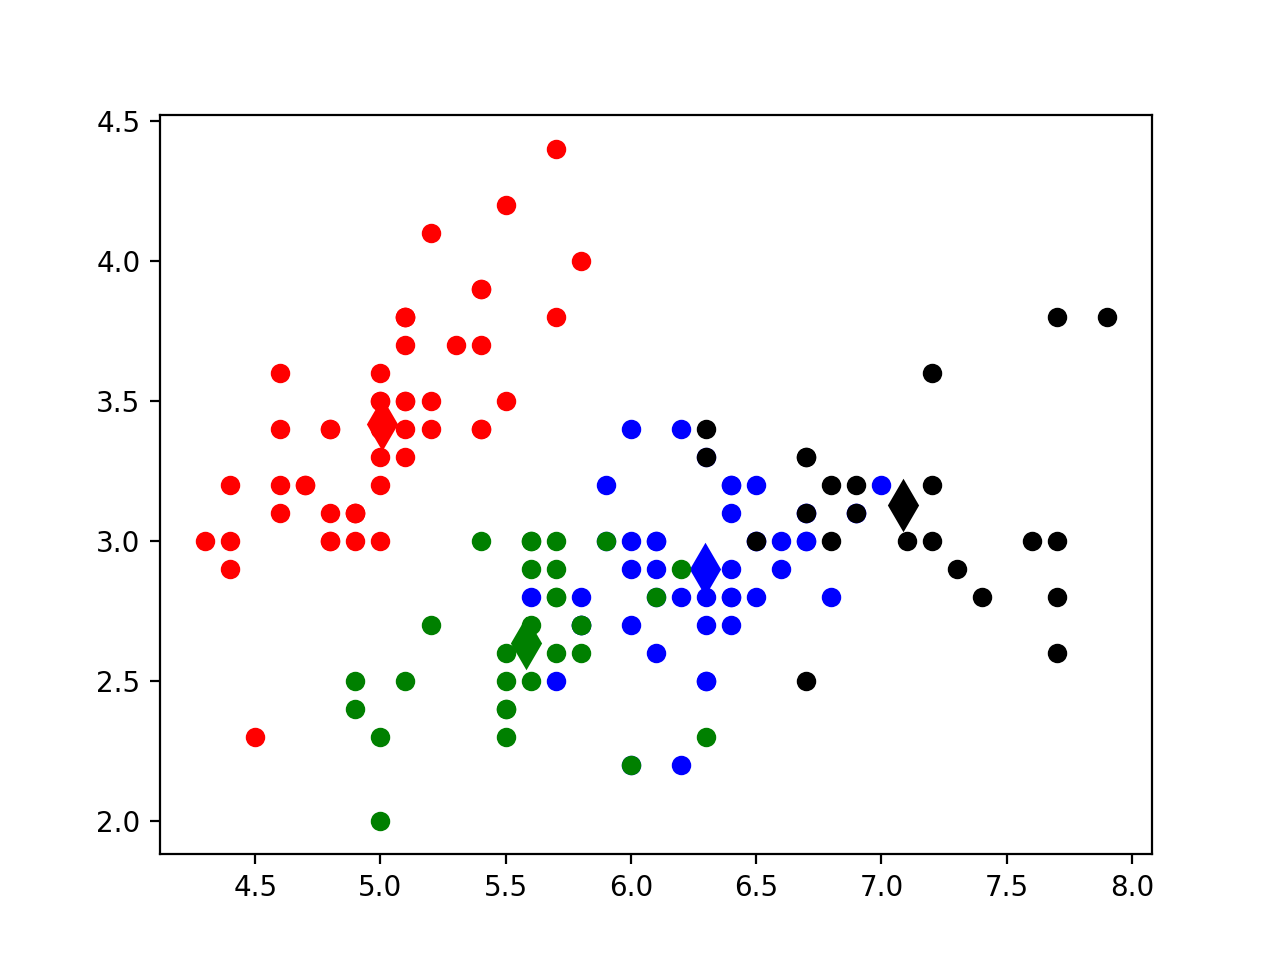
\includegraphics[width=1.7in]{image/f16}
            \end{minipage}% 
        }%
        \subfigure[fig2.]{
            \begin{minipage}[t]{0.25\linewidth}
            \centering
            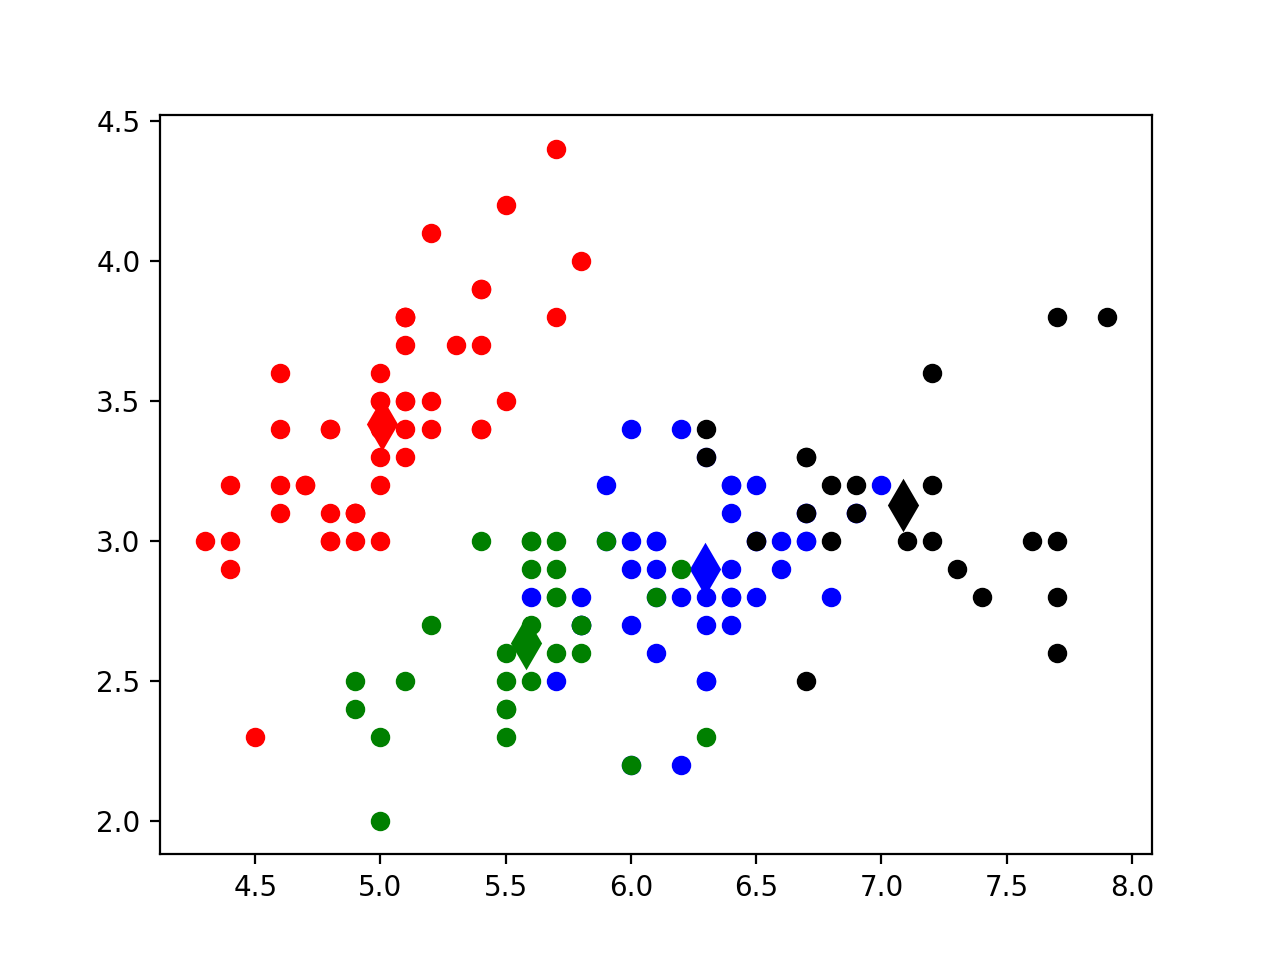
\includegraphics[width=1.7in]{image/f15}
            \end{minipage}% 
            }%
        \subfigure[fig3.]{
            \begin{minipage}[t]{0.25\linewidth}
            \centering
            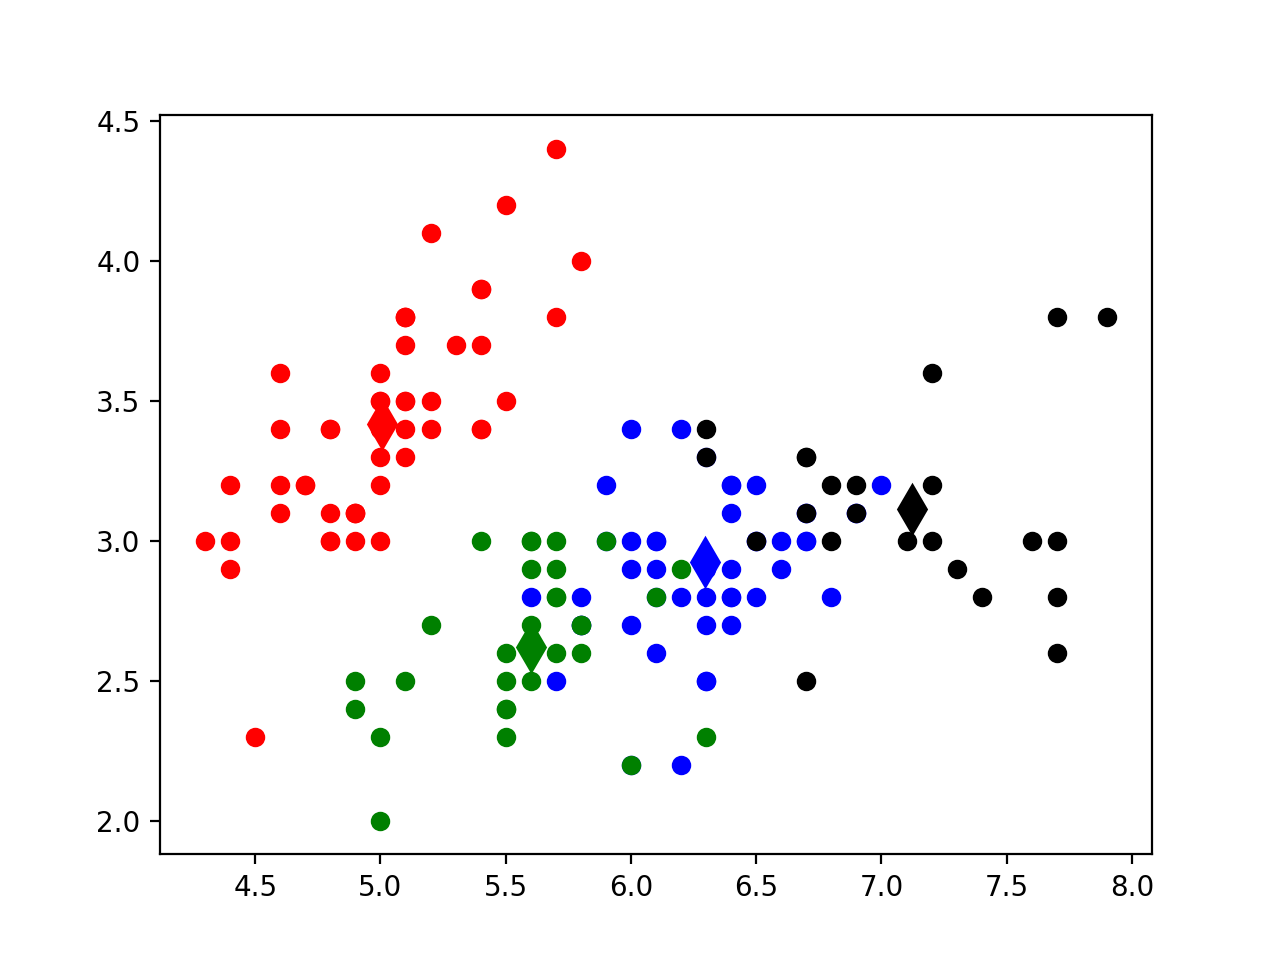
\includegraphics[width=1.7in]{image/f14}
            \end{minipage}% 
        }% 
        \subfigure[fig4.]{
            \begin{minipage}[t]{0.25\linewidth}
            \centering
            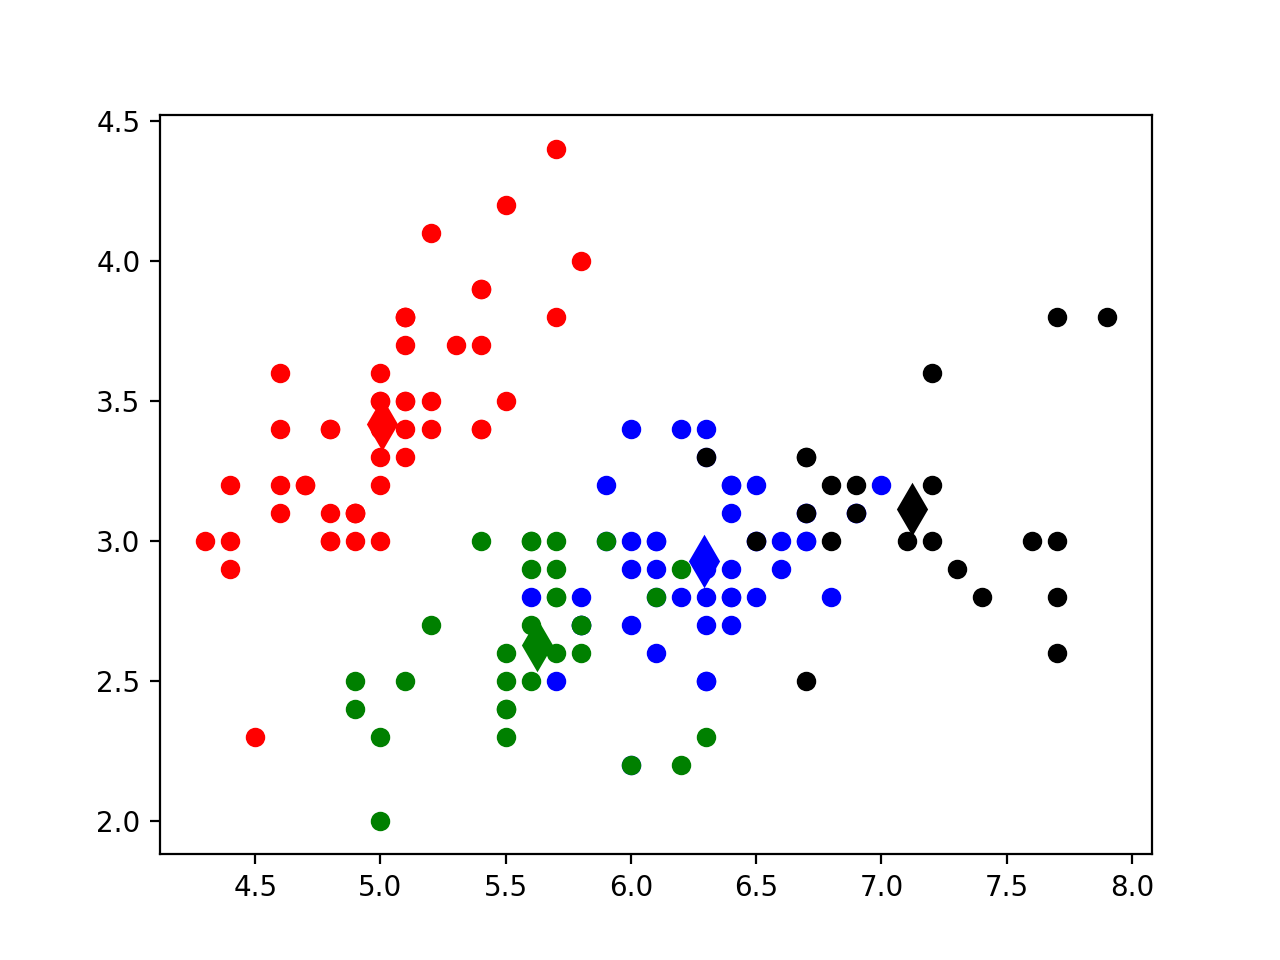
\includegraphics[width=1.7in]{image/f13}
            \end{minipage}% 
        }%
        \\
        \subfigure[fig5.]{
            \begin{minipage}[t]{0.25\linewidth}
            \centering
            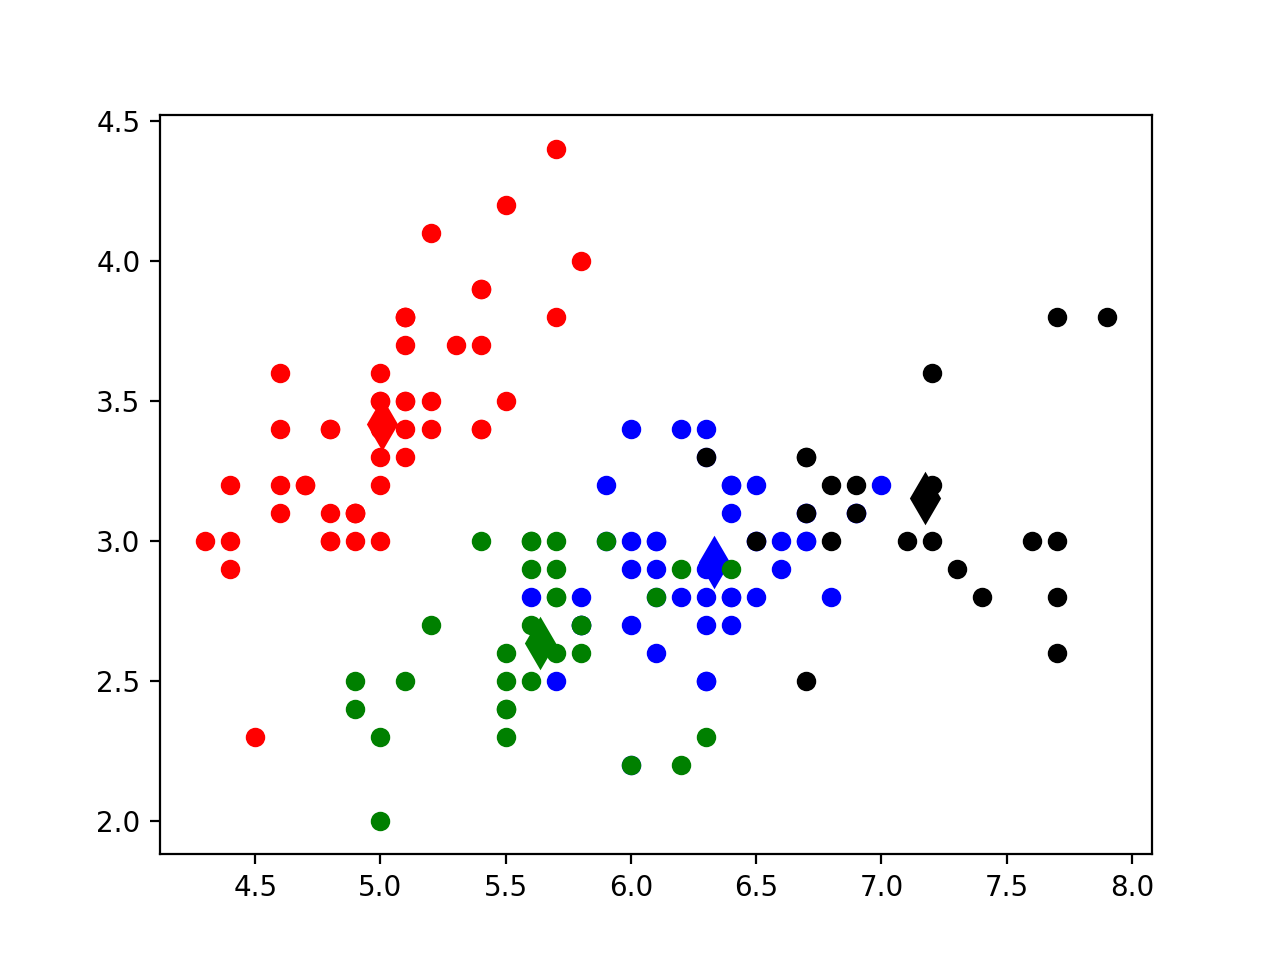
\includegraphics[width=1.7in]{image/f12}
            \end{minipage}% 
        }%
        \subfigure[fig6.]{
            \begin{minipage}[t]{0.25\linewidth}
            \centering
            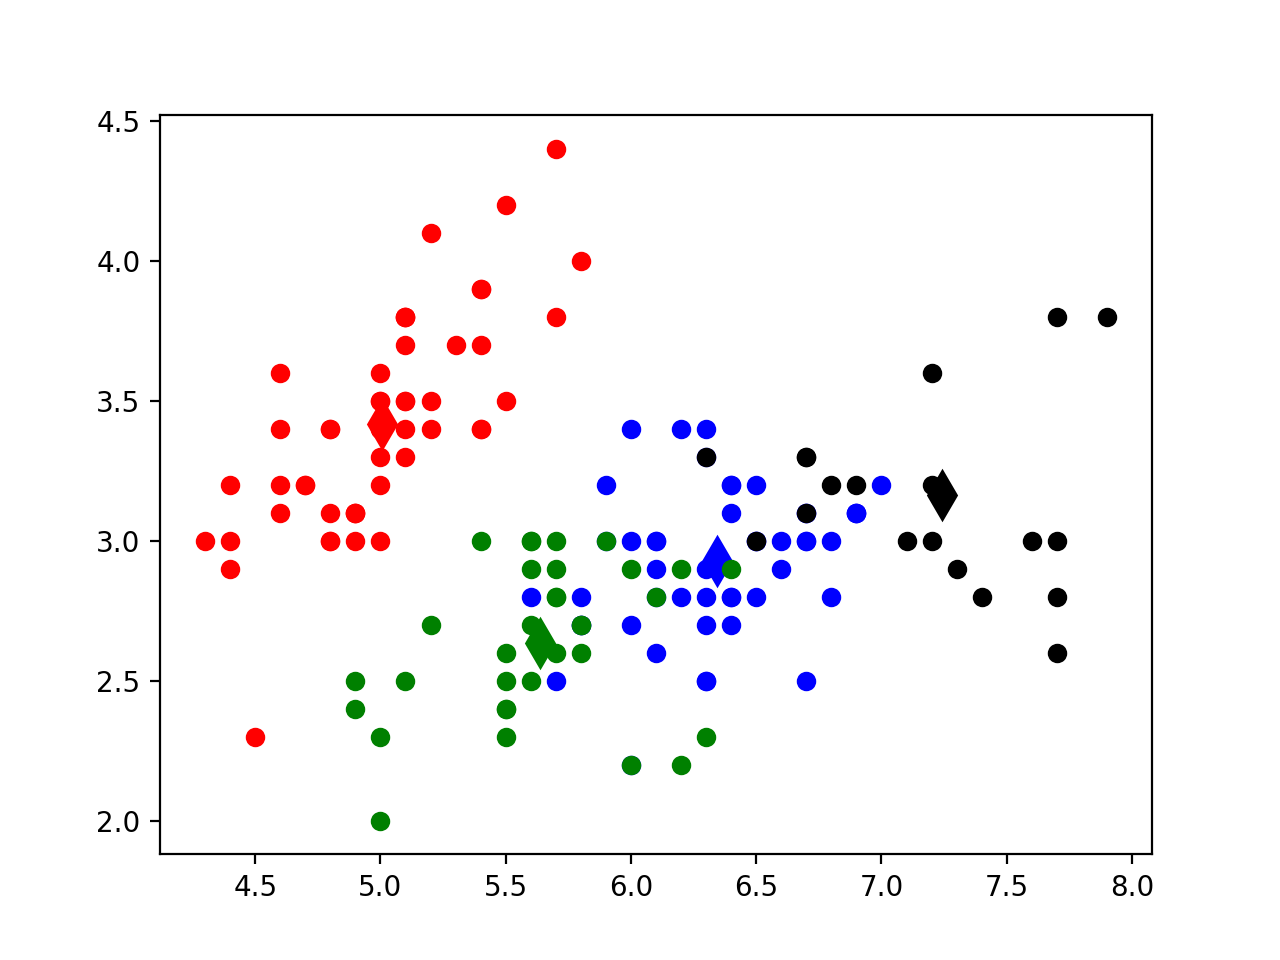
\includegraphics[width=1.7in]{image/f11}
            \end{minipage}% 
            }%
        \subfigure[fig7.]{
            \begin{minipage}[t]{0.25\linewidth}
            \centering
            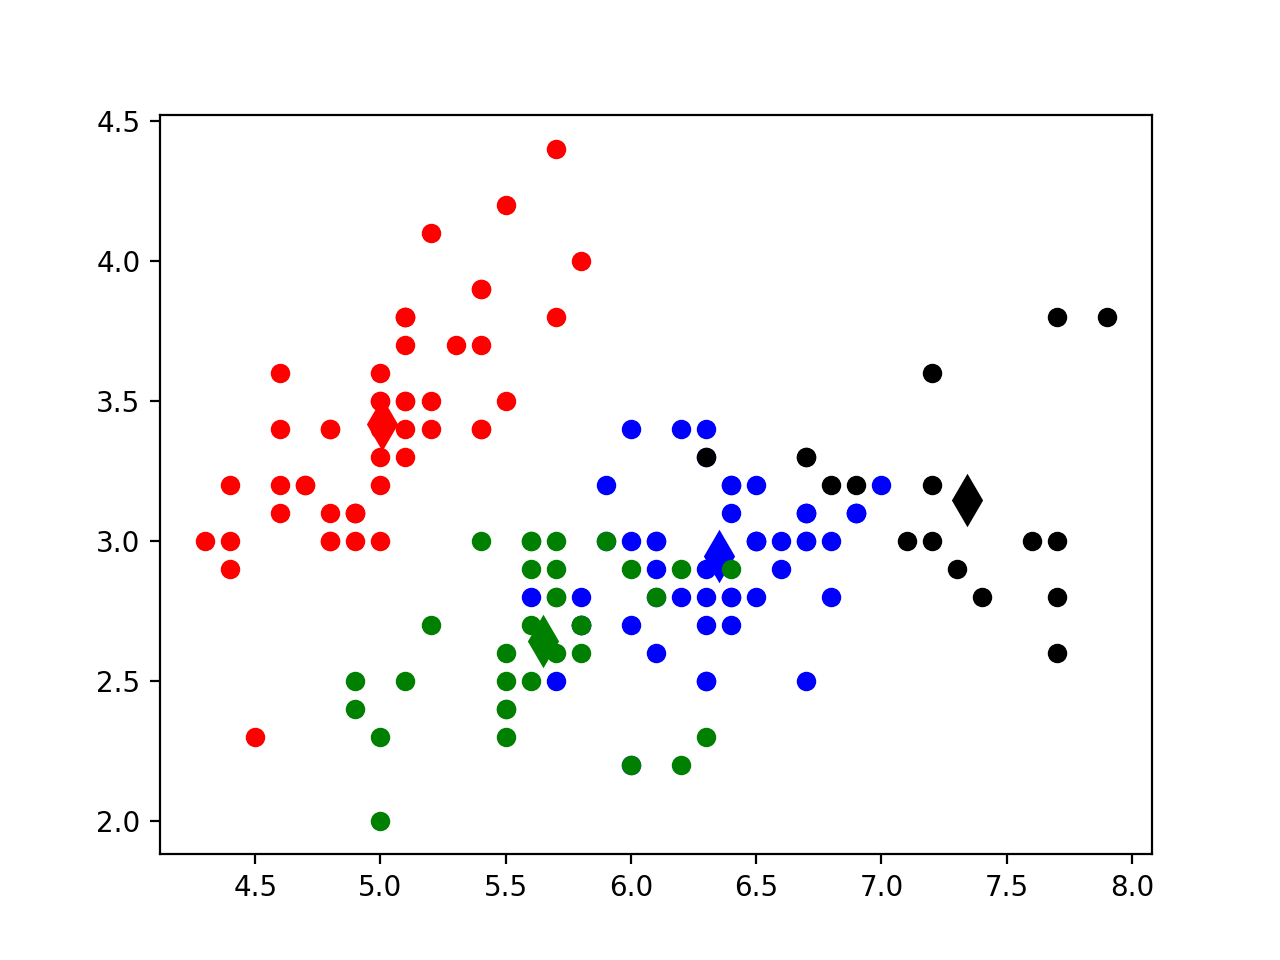
\includegraphics[width=1.7in]{image/f10}
            \end{minipage}% 
        }% 
        \subfigure[fig8.]{
            \begin{minipage}[t]{0.25\linewidth}
            \centering
            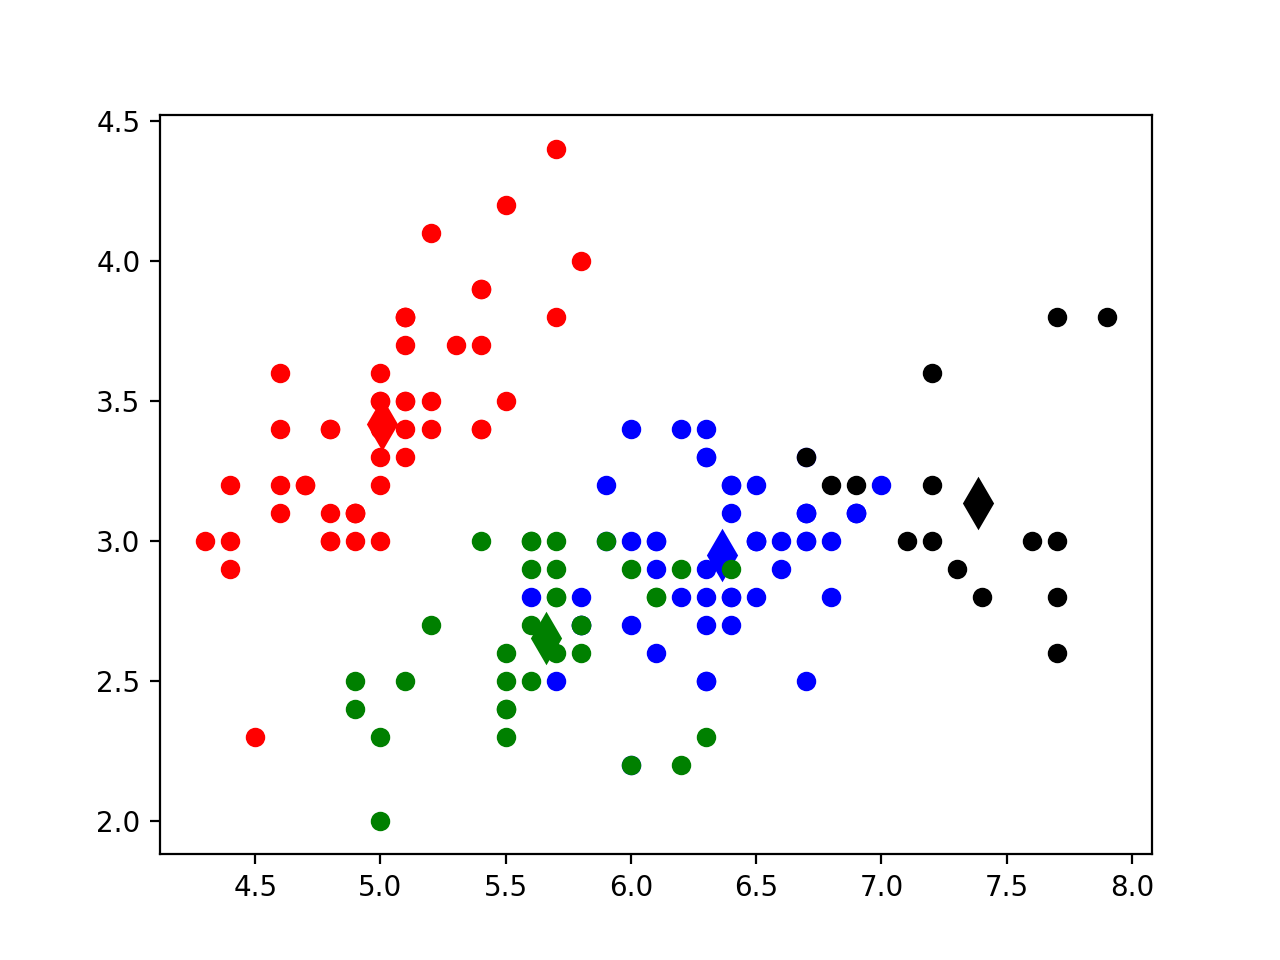
\includegraphics[width=1.7in]{image/f9}
            \end{minipage}% 
        }%
        \\
        \subfigure[fig9.]{
            \begin{minipage}[t]{0.25\linewidth}
            \centering
            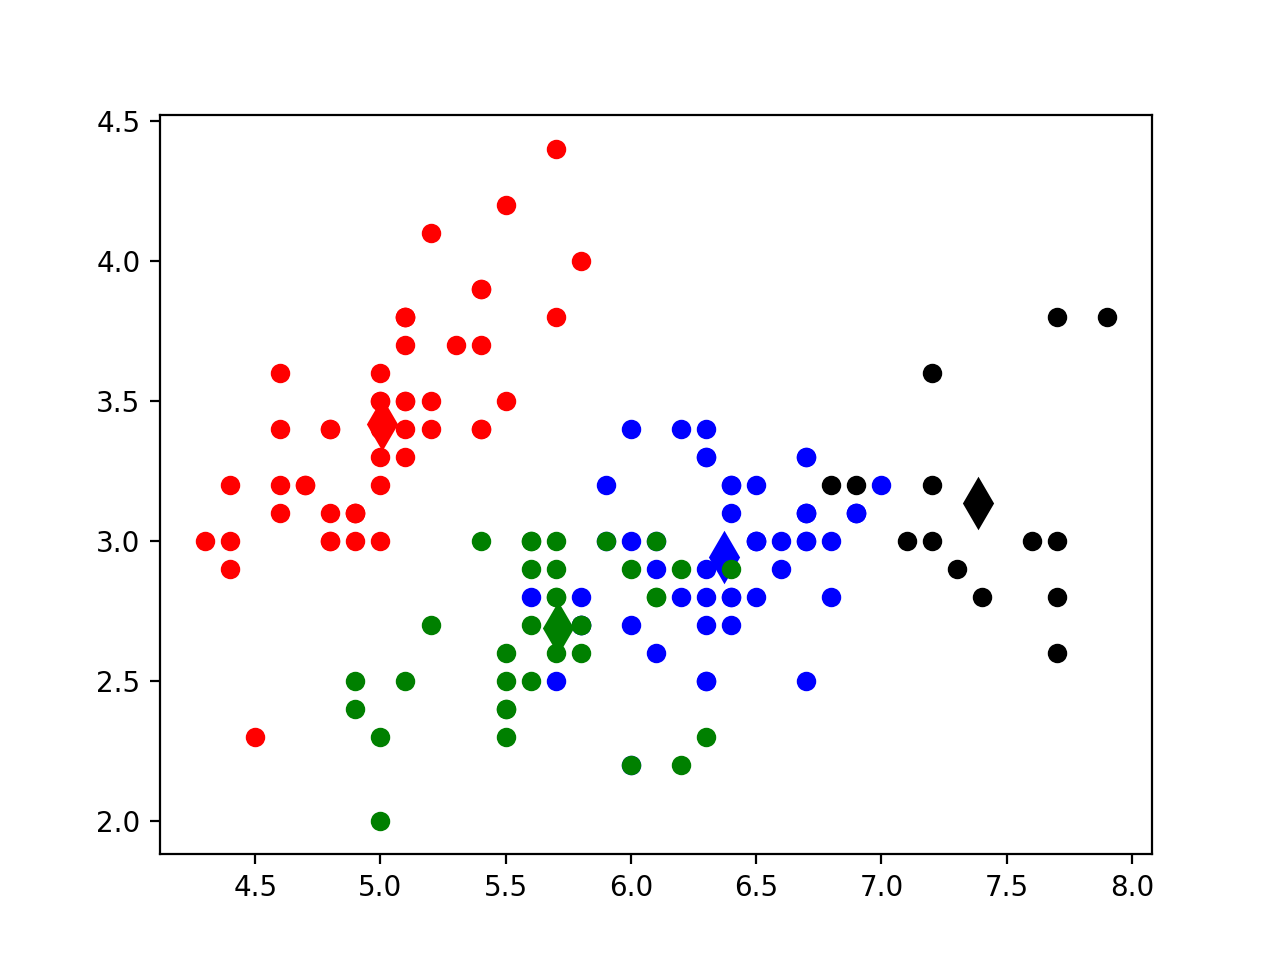
\includegraphics[width=1.7in]{image/f8}
            \end{minipage}% 
        }%
        \subfigure[fig10.]{
            \begin{minipage}[t]{0.25\linewidth}
            \centering
            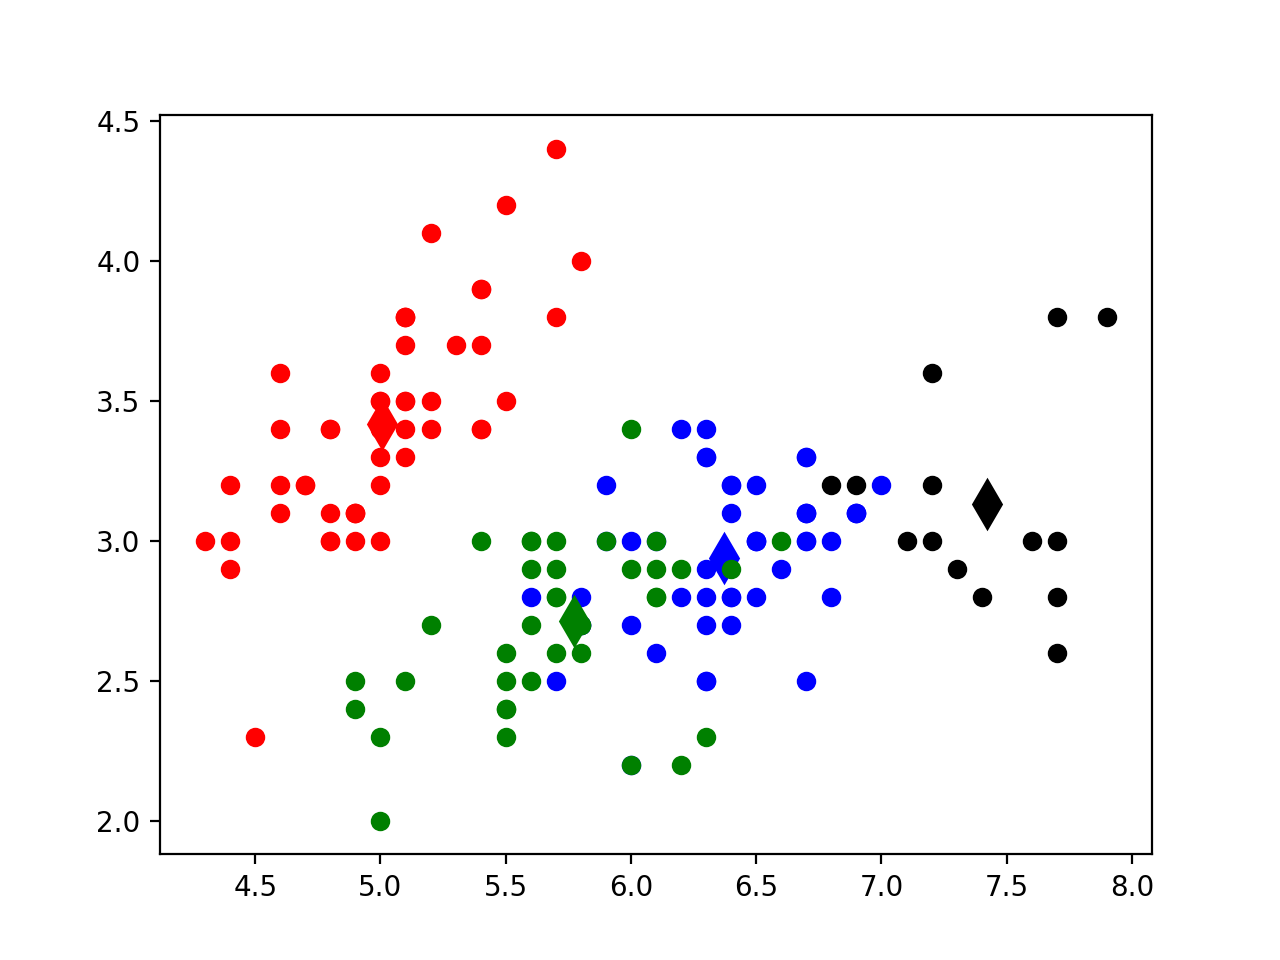
\includegraphics[width=1.7in]{image/f7}
            \end{minipage}% 
            }%
        \subfigure[fig11.]{
            \begin{minipage}[t]{0.25\linewidth}
            \centering
            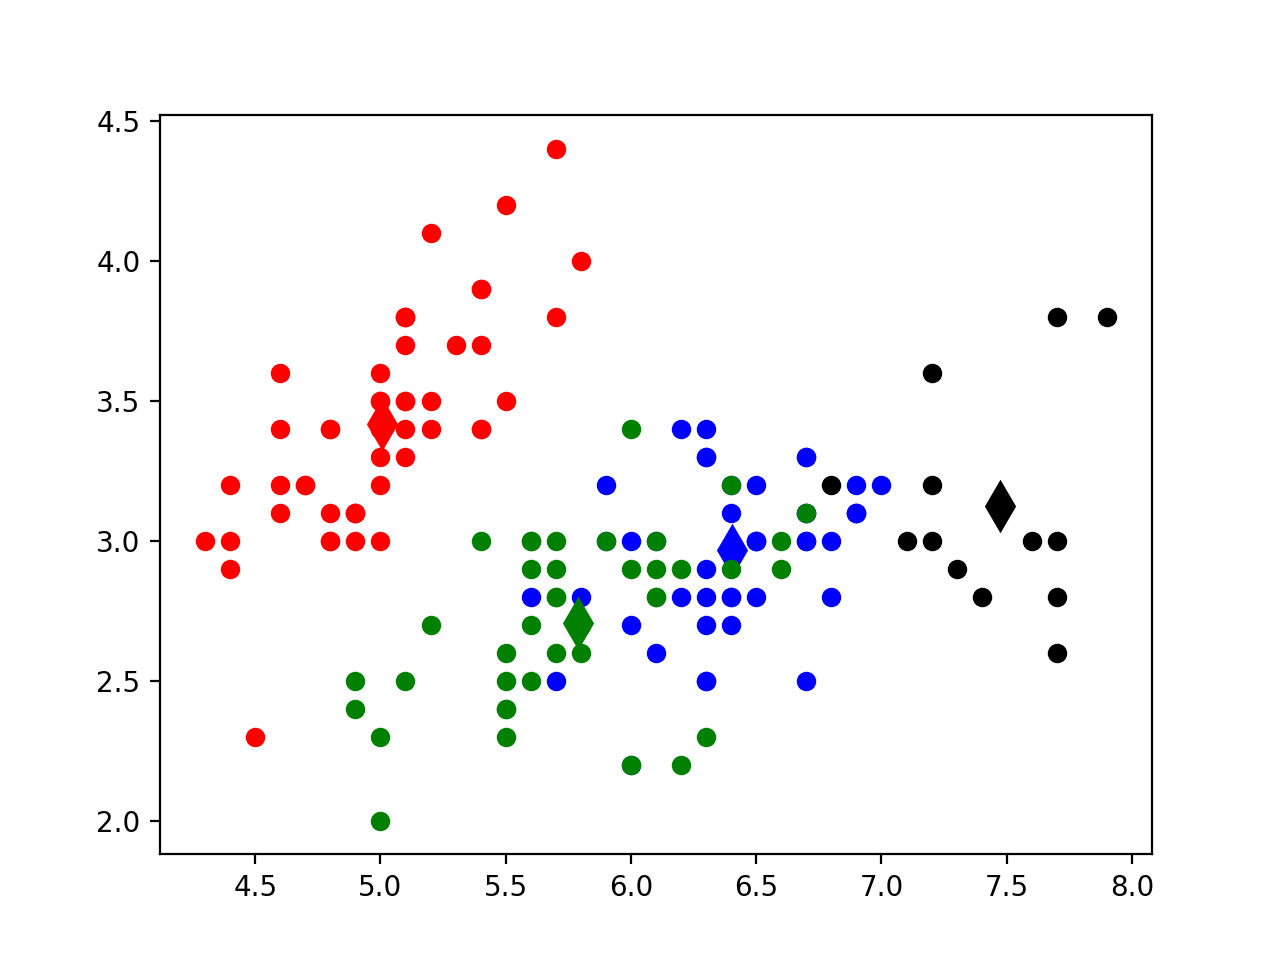
\includegraphics[width=1.7in]{image/f6}
            \end{minipage}% 
        }% 
        \subfigure[fig12.]{
            \begin{minipage}[t]{0.25\linewidth}
            \centering
            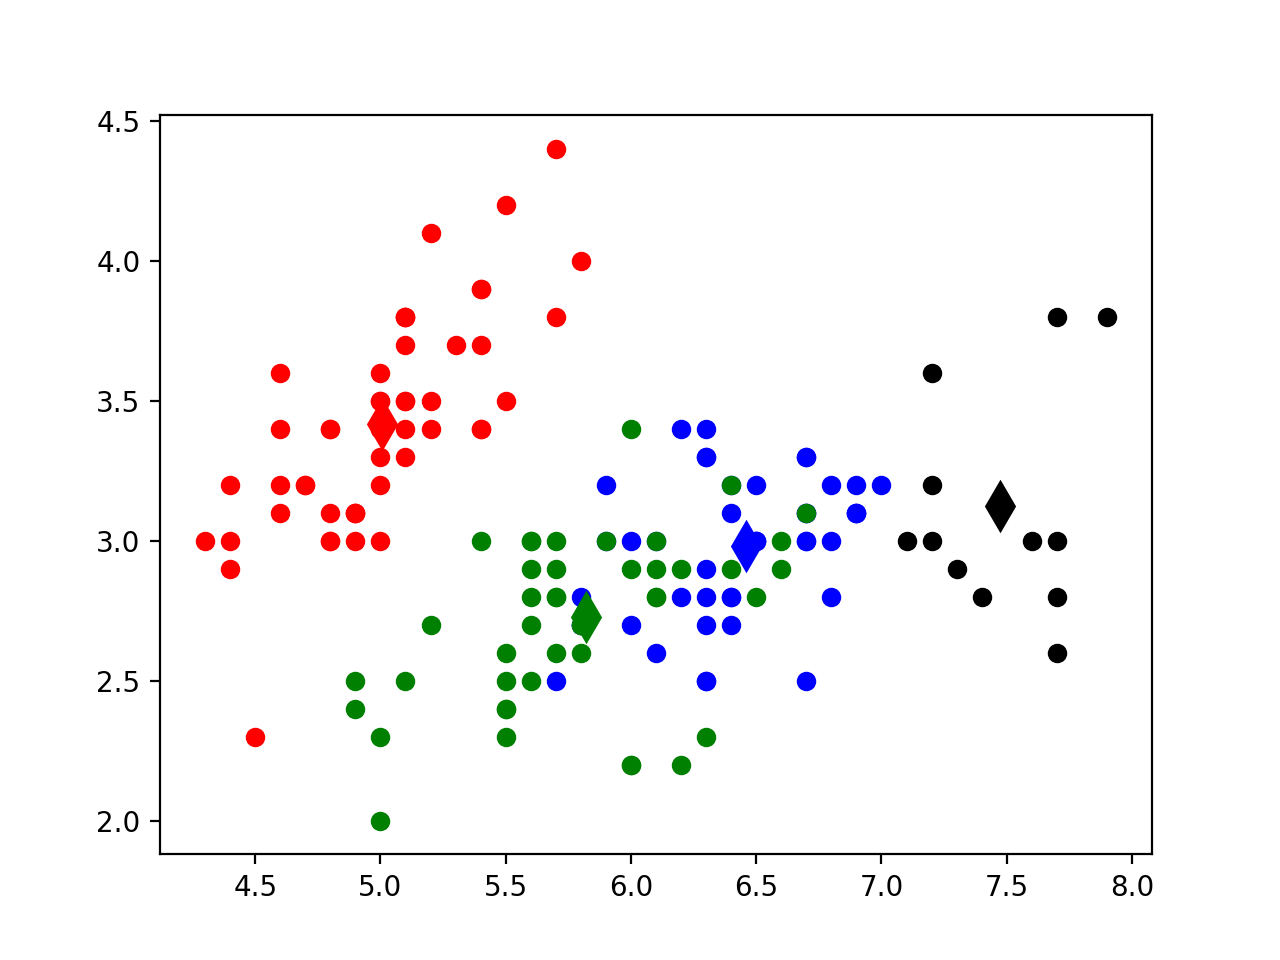
\includegraphics[width=1.7in]{image/f5}
            \end{minipage}% 
        }%
        \\
        \subfigure[fig13.]{
            \begin{minipage}[t]{0.25\linewidth}
            \centering
            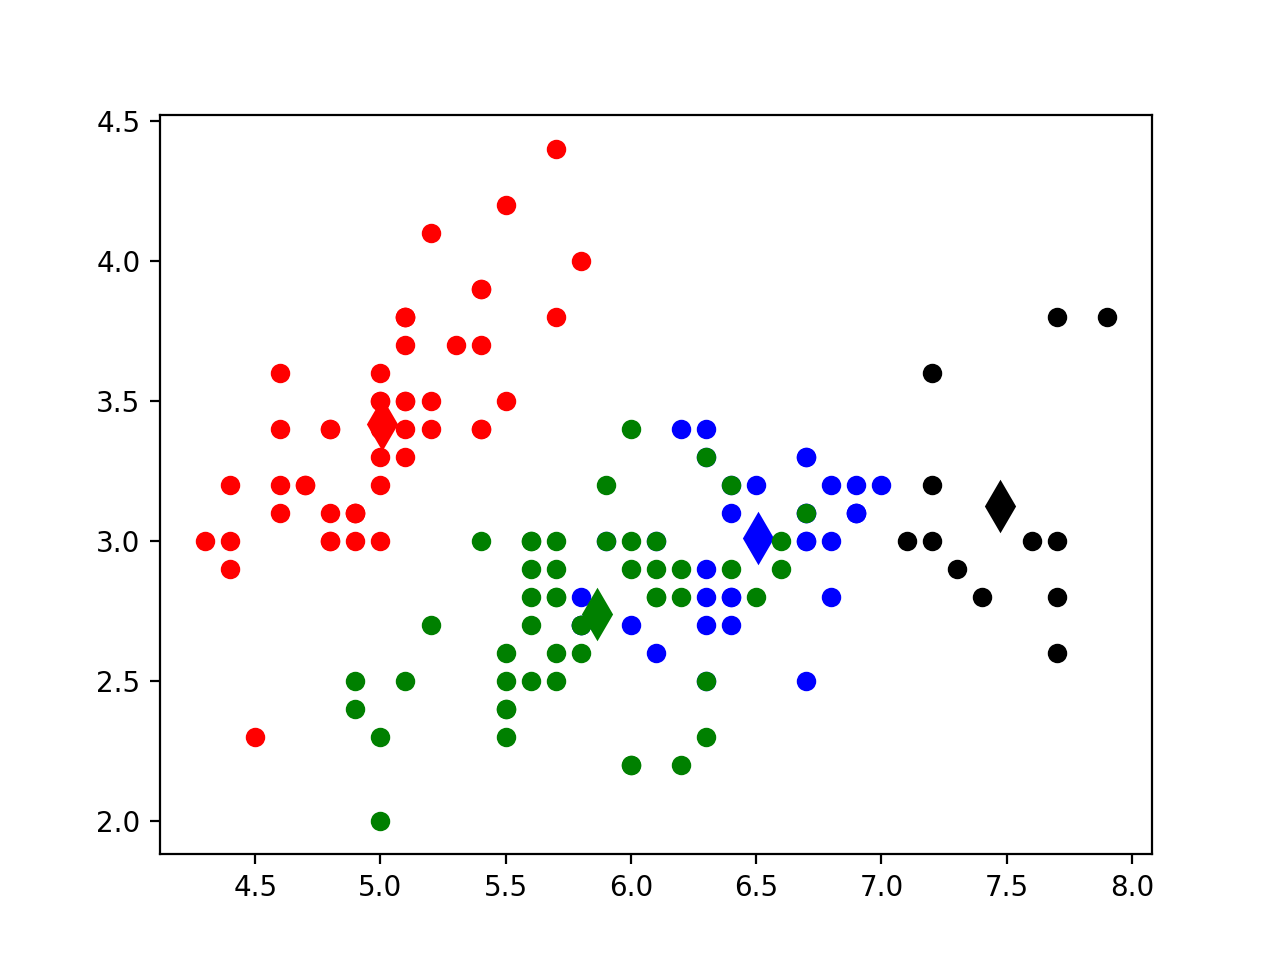
\includegraphics[width=1.7in]{image/f4}
            \end{minipage}% 
        }%
        \subfigure[fig14.]{
            \begin{minipage}[t]{0.25\linewidth}
            \centering
            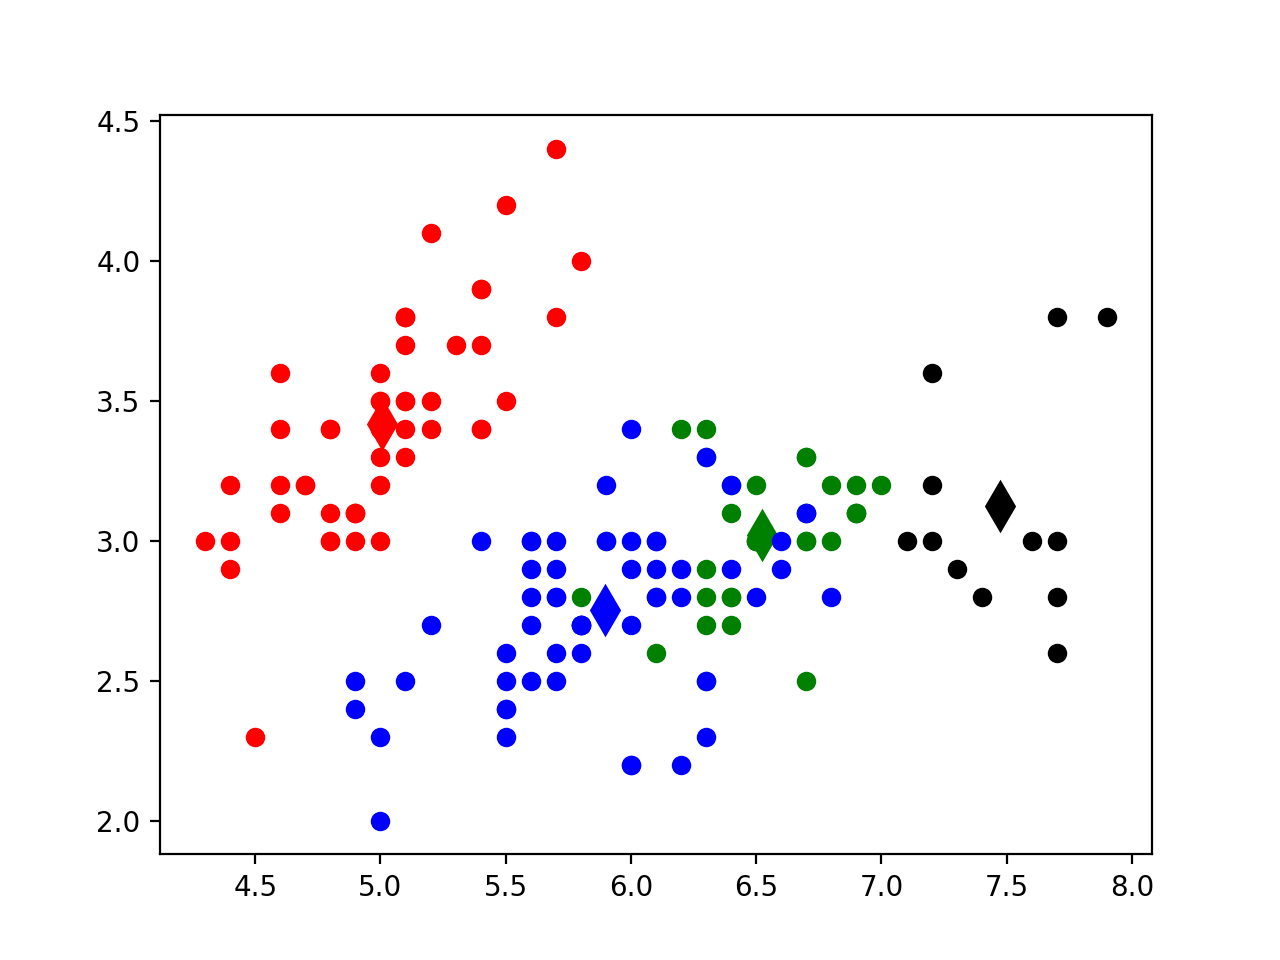
\includegraphics[width=1.7in]{image/f3}
            \end{minipage}% 
            }%
        \subfigure[fig15.]{
            \begin{minipage}[t]{0.25\linewidth}
            \centering
            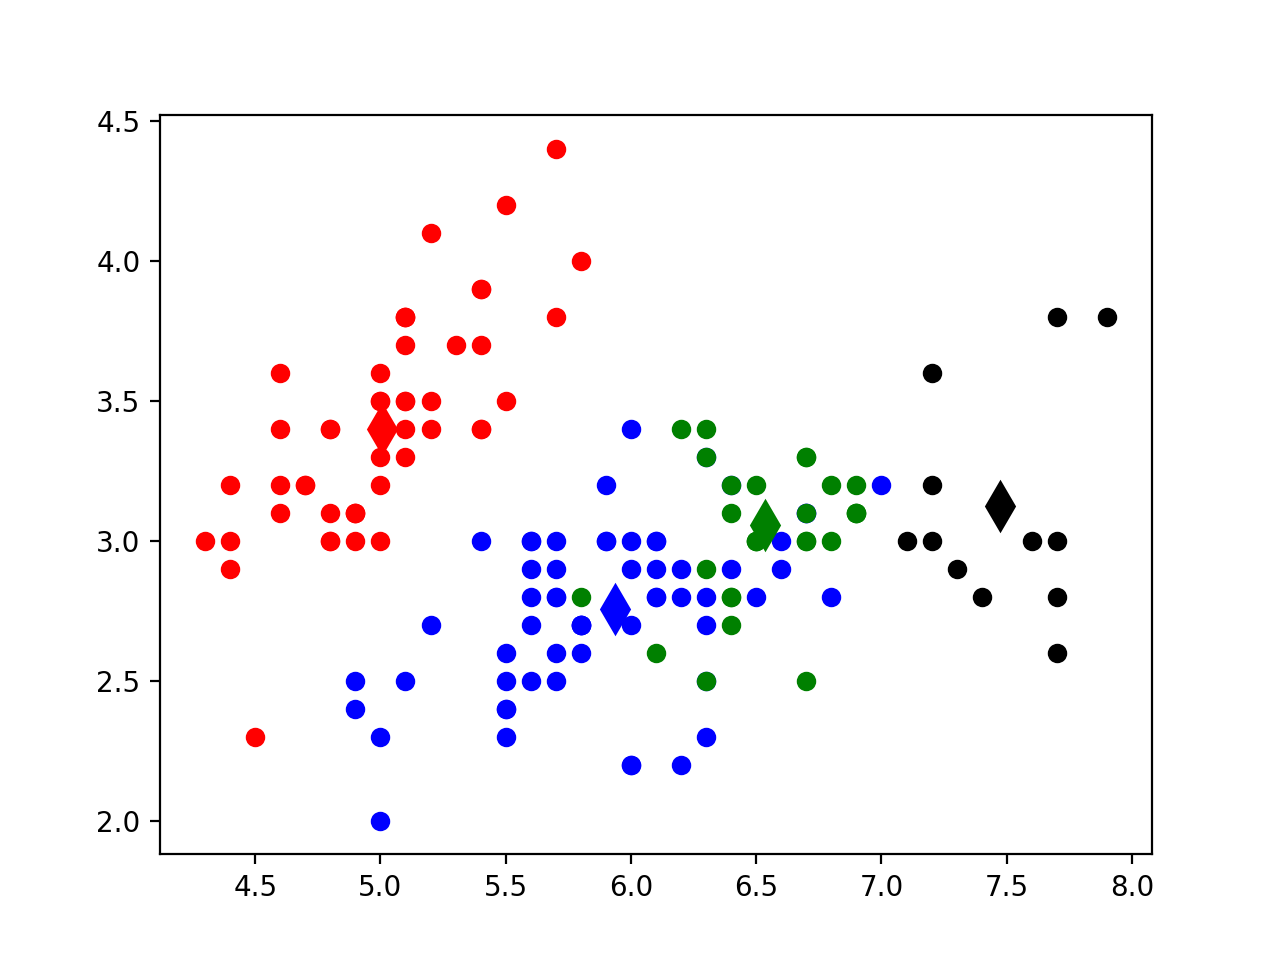
\includegraphics[width=1.7in]{image/f2}
            \end{minipage}% 
        }% 
        \subfigure[fig16.]{
            \begin{minipage}[t]{0.25\linewidth}
            \centering
            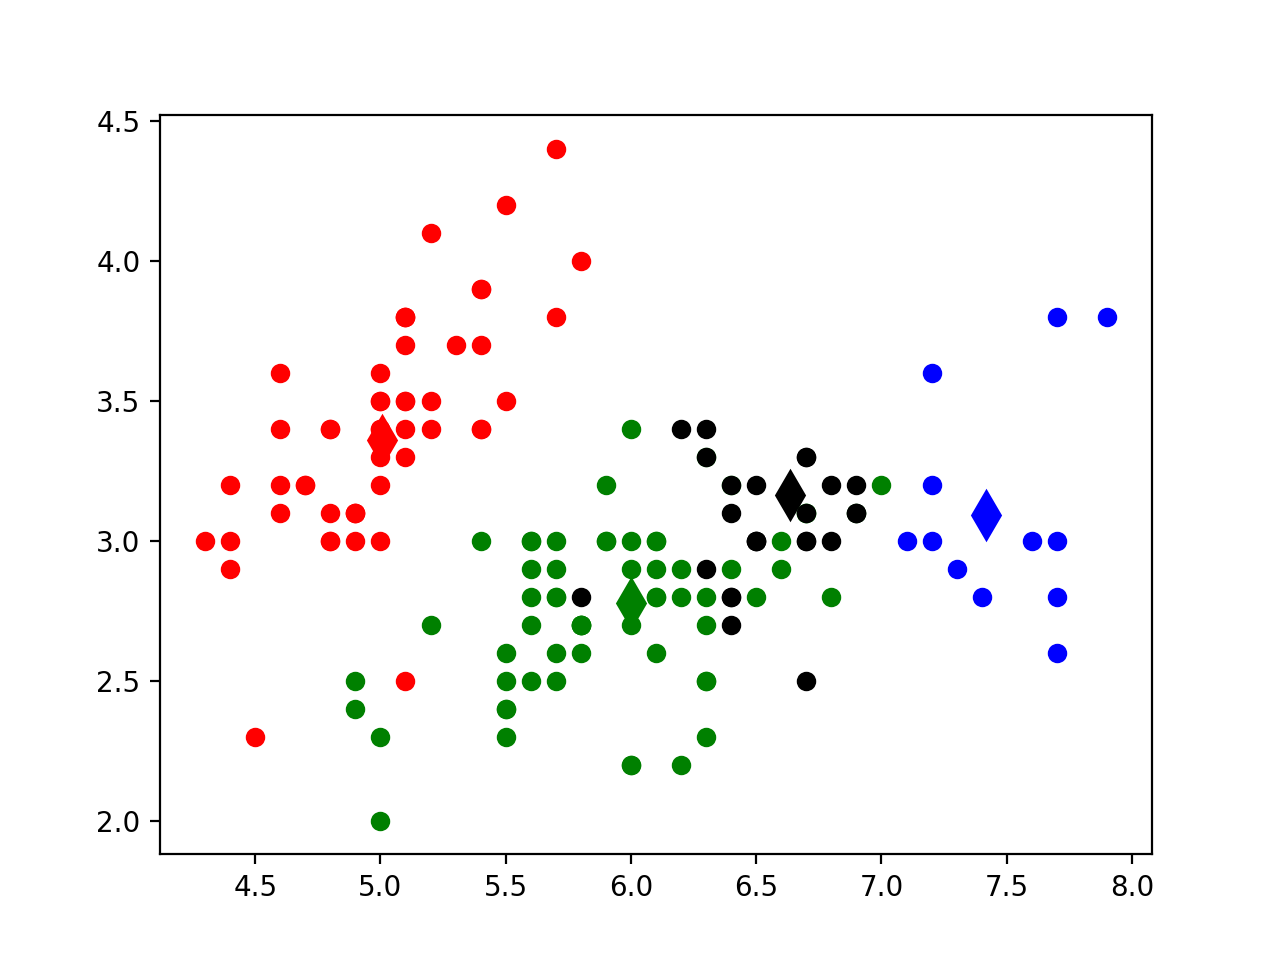
\includegraphics[width=1.7in]{image/f1}
            \end{minipage}% 
        }%
        \caption{Clustering of Iris dataset}
    \end{figure} 
\end{homeworkProblem}
\end{document}
